\section{Leveraging \smt to Build Transparent Multithreaded State Machine Replication} \label{sec:replication}

This section proposes \msmr, a new system that provides 
state-machine replication service to multi-threaded server programs 
transparently without modifying or annotating these programs.
   
\subsection{Introduction} \label{sec:rep-intro}


%% P1
Stable-machine replication (or SMR) has become a popular and critical fault-tolerance 
technique [cite], because the cloud computing trend requires server programs to be 
highly available. Typically, a SMR system leverages \paxos to ensure 
consensus on the same totally ordered sequence on inputs among replicas, so that 
active replicas (with each runs one thread) perform the same sequence of state 
transitions and produce the same sequence of outputs.

%% P2
Unfortunately, despite much efforts from academia and industry, it is still 
insurfficient to build SMR for multi-threaded server programs on multi-core 
hardware transparently, and a key reason is even all replicas are working 
correctly, the thread interleavings (or schedules) in different replicas may 
artificially diverge at runtime and leading to diverged states. To address this 
problem, existing SMR systems either restrict the number of threads running in each 
replica to be only one [cite], or require developers to manually annotate all shared states 
among threads [cite], which may be time consuming and error prone.

%% P3
One may consider that recent advances on stable and deterministic multithreading 
[cite] or deterministic replay [cite, Rex] can simply address the above state 
divergence problem, because these systems can a fixed logical clock rather than in 
a physical clock for each inter-thread communication (\eg, mutex\_lock).
However, although these techniques are promising, as we will discuss further in the following sections, 
these techniques face two fundamental challenges. First, network delay may 
causes input request to arrive at different replicas at various physical 
clocks, and deterministic/stable multithreading systems have to 
convert these clocks to a consistent logical clocks of these requests in their own schedules. Second, 
to achieve good performance, moden SMR systems allow read-only request to 
bypass the consensus and be processed in local replicas fastly. However, this read-only 
requests may change the internal logical clocks or states of a program, 
fundamentally breaking all these threading systems (\eg, replay may fail 
because different replicas have served different read-only requests [cite Rex]).

%% P4
To address these two challenges and let stable and deterministic 
multithreading enable transparent SMR for multi-core servers, we propose \msmr.
In order to support general multi-threaded server programs, \msmr chooses the 
POXIS socket operations (\eg, connect(), accept(), send(), and recv()) as the 
requests for consensus, and chooses a pracitcal \smt runtime system called 
\parrot to reduce the number of schedules in multi-threaded programs. The key 
novelty of \msmr is a novel algorithm called XXX on addressing the timing 
challenge: this algorithm works seamlessly with general \smt or \dmt runtime systems, 
and convert the timing problem into a input generation problem, greatly simplifying the consensus on 
request timings and have fast performance. To support read-only optimization 
in modern SMR applications, we proposes our new approach that can soundly 
detect internal state divergences in the server programs and safely rollback.

%% P5
An critical challenge for the practicalness of transparent SMR is: \msmr must 
support systematic checkpoint and recovery. One major limitation of existing SMR 
frameworks [cite Rex] is: they often require developers to write their own 
customized checkpointing and recovery logic for each application, adding lots 
of burdens to the developers and making SMR deployments tedious and 
error prone [cite MongoDB]. To address this pracitcal challenge, \msmr builds a 
systematic checkpoint mechanism that supports systematic and transparent 
checkpointing applications, including the application states of file systems, memory, and CPU registers.

%% P6
In addition to enabling transparent SMR on multi-core servers, \msmr have other 
broad applications. First, by carefully designing the consensue interface on 
the socket operation level, \msmr can also benefit transparent replication of 
single-threaded server applications. Second, \msmr enables heavyweight concurrency analysis at 
deployment, which was impossible before. In order to improve reliability and 
security of multi-threaded programs, both academia and industry have built 
sophisticate analysis tools to detect runtime misbehavior (\eg, data race detections, 
data flow tracking). However, these tools often perform heavyweight 
analysis and introduce prohibitive slow down (\eg, running a Googld dynamic data race detector 
TSan carried with gcc-4.8 typically have 30x to 100x slowdown). Fortunately, by 
levegaring the transparent SMR in \msmr, these tools can now run on a dedicated 
replica without hurting the primary to server requests much, greatly benefiting 
these tools for deployment and adoption.

%% P7
\msmr is easy to deploy.
By integrating with a pracitcal \msmr runtime system \parrot and 
performing consensus on the socket interface, ,
and the server applications running with \msmr 
only requires to be Pthreads compatible, x86 binary, and uses socket operations 
to accept requests (\ie, we currently do not support libevent based servers). 
Although \parrot ignores memory level schedule divergence, by leveraging the replication architecture,
\msmr can also practically capture  this kind of divergence (\eg, caused by data races) by running a 
race detector on a dedicated replica.

%% P8
In evaluation, we will focus on these questions. First, can \msmr support a diverse 
set of popular multi-threaded server programs and have reasonable runtime overhead? we plan to evaluate \msmr with 
over 10 server programs, ranging from web servers, to database servers, and to 
key value store servers, and measure their performance running with and without \msmr.
Second, can \msmr practically capture memory level divergence with a dedicated 
replica running data race detectors? We plan to collect results on this track. 
Third, what is the performance benefit and breakdown of our read-only 
optimization approach? Fourth, what is the performance and functionality impact 
by injecting realisitic replica failures and network partitions?

  
%% The cloud computing trend requires services on the web to be highly available. In order to 
%% provide high availability, the state machine replication (or SMR) approach has 
%% become popular. In this approach, a state machine, which runs a single threaded 
%% service that always produce the same output on the same input request, 
%% is invoked on a number of nodes, and a \paxos protocal enforces the same 
%% sequence (total order) of requests for each state machine. \paxos can safely ensure
%% the whole system consistently execute the same sequence of requests as long as 
%% no more than half of nodes are down, providing high robustness and availability.


%% Unfortunately, despite much efforts, the benefit of this SMR approach still can 
%% be enjoyed by general web services (\eg, server programs) because of two 
%% reasons. First, only work with some specific components of an application with 
%% specific interface, require expert knowledge on 
%% distributed systems, has no a systematic checkpiont and recovery techniques for 
%% the state machines. Second, due to the ``single threaded" requirement on each 
%% state machine, even existing applicaions with SMR components can not 
%% benefit from the performance of the rising multi-core trend.

%% Unfortunately, despite much effort from academia and industry, it is still 
%% insufficient for software vendors to provide practical state machine 
%% replication service to general applications, because of two challenges. First, existing 
%% state machine replication techniques typically require developers to replicate 
%% a specific subset of program states (with APIs) instead of the whole program 
%% states, which requires strong distributed sytems expert knowledge, hard to 
%% maintain with the rest of the applications, and error prone 
%% (Todo: cite the MongoDB exmample). Second, existing SMR infrastructures assume all 
%% replicas always run the same schedule for the same input, pracitally restricing 
%% the number of running threads to be only one and preventing them fully leverage the 
%% power of the multi-core hardware.

%% Why is this problem hard? Two parts: research challenge (limitations of 
%% existing approaches) and practical 
%% challenges (performance, read-only optimization).


%% This article made two major contributions towards building practical state-
%% machine replications for multithreaded programs. First, how to reach 
%% consensus on general network inputs (including input values and timings) 
%% across replicas. Second, how to perform read-only 
%% optimization for general applications, which is hard, because some 
%% semantically read only operations (such as get() in key-value store and GET 
%% in http servers) may modify states of server programs.

%% Our system is the first system on building practical state-machine 
%% replications for general multi-threaded programs. Todo: how it works: reach 
%% consensus on general socket operations, LD\_PRELOAD, transparent (do not need 
%% to annotate shared states in a program) replications for servers.

%% Introduce the fault-tolerance and performance features (guarantees) of our 
%% system.

%% Todo: usage scenarios (what kinds of applications can benefit from \msmr) and
%% fundamental assumptions (what assumptions to make: \eg, race free) of \msmr. 
%% Overall, all applications that can benefit from replicated fault tolerence (or 
%% high availability) and 
%% multi-core performance can benefit from our system, and we mainly focus on 
%% server programs. Regarding assumptions, currently we don't need this, because 
%% even for data races, we can simply run a stock race detector at one replica 
%% (with little performance impact) and 
%% flags warnings whenever we detect races (benign or harmful), and developers can 
%% diagnose and fix that.

%% Practical highlights of our system: evaluated a good range of popular server 
%% programs, ranging from web servers, data base servers, key-value stores, and 
%% popular utility programs. Todo: performance highlights, recovery highlights.

\subsection{\msmr: A Pracitcal SMR sytem for general multithreaded programs} \label{sec:rep-msmr}
This section first introduces the \msmr architecture, and then describes how it 
ensure consensus on socket APIs, and then presents our design on read-only 
optimization.

\subsubsection{\msmr architecture} \label{sec:rep-arch}

Figure XXX shows the \msmr architecture in each node. Each node starts with a proxy, 
which is a \paxos daemon (\S\ref{sec:rep-consensus}), and each proxy forks a child to execute an 
application (\eg, a web server) running with a \smt tool. The proxy has a logger module to 
persistently manage executed operations, and it also has a read optimizer (\S\ref{sec:rep-readonly})
module to perform read optimization. A checkpoint (\S\ref{sec:rep-checkpoint}) module sits on both 
application site and kernel site in order to checkpoint execution states of each application.

\begin{figure}[t]
\centering
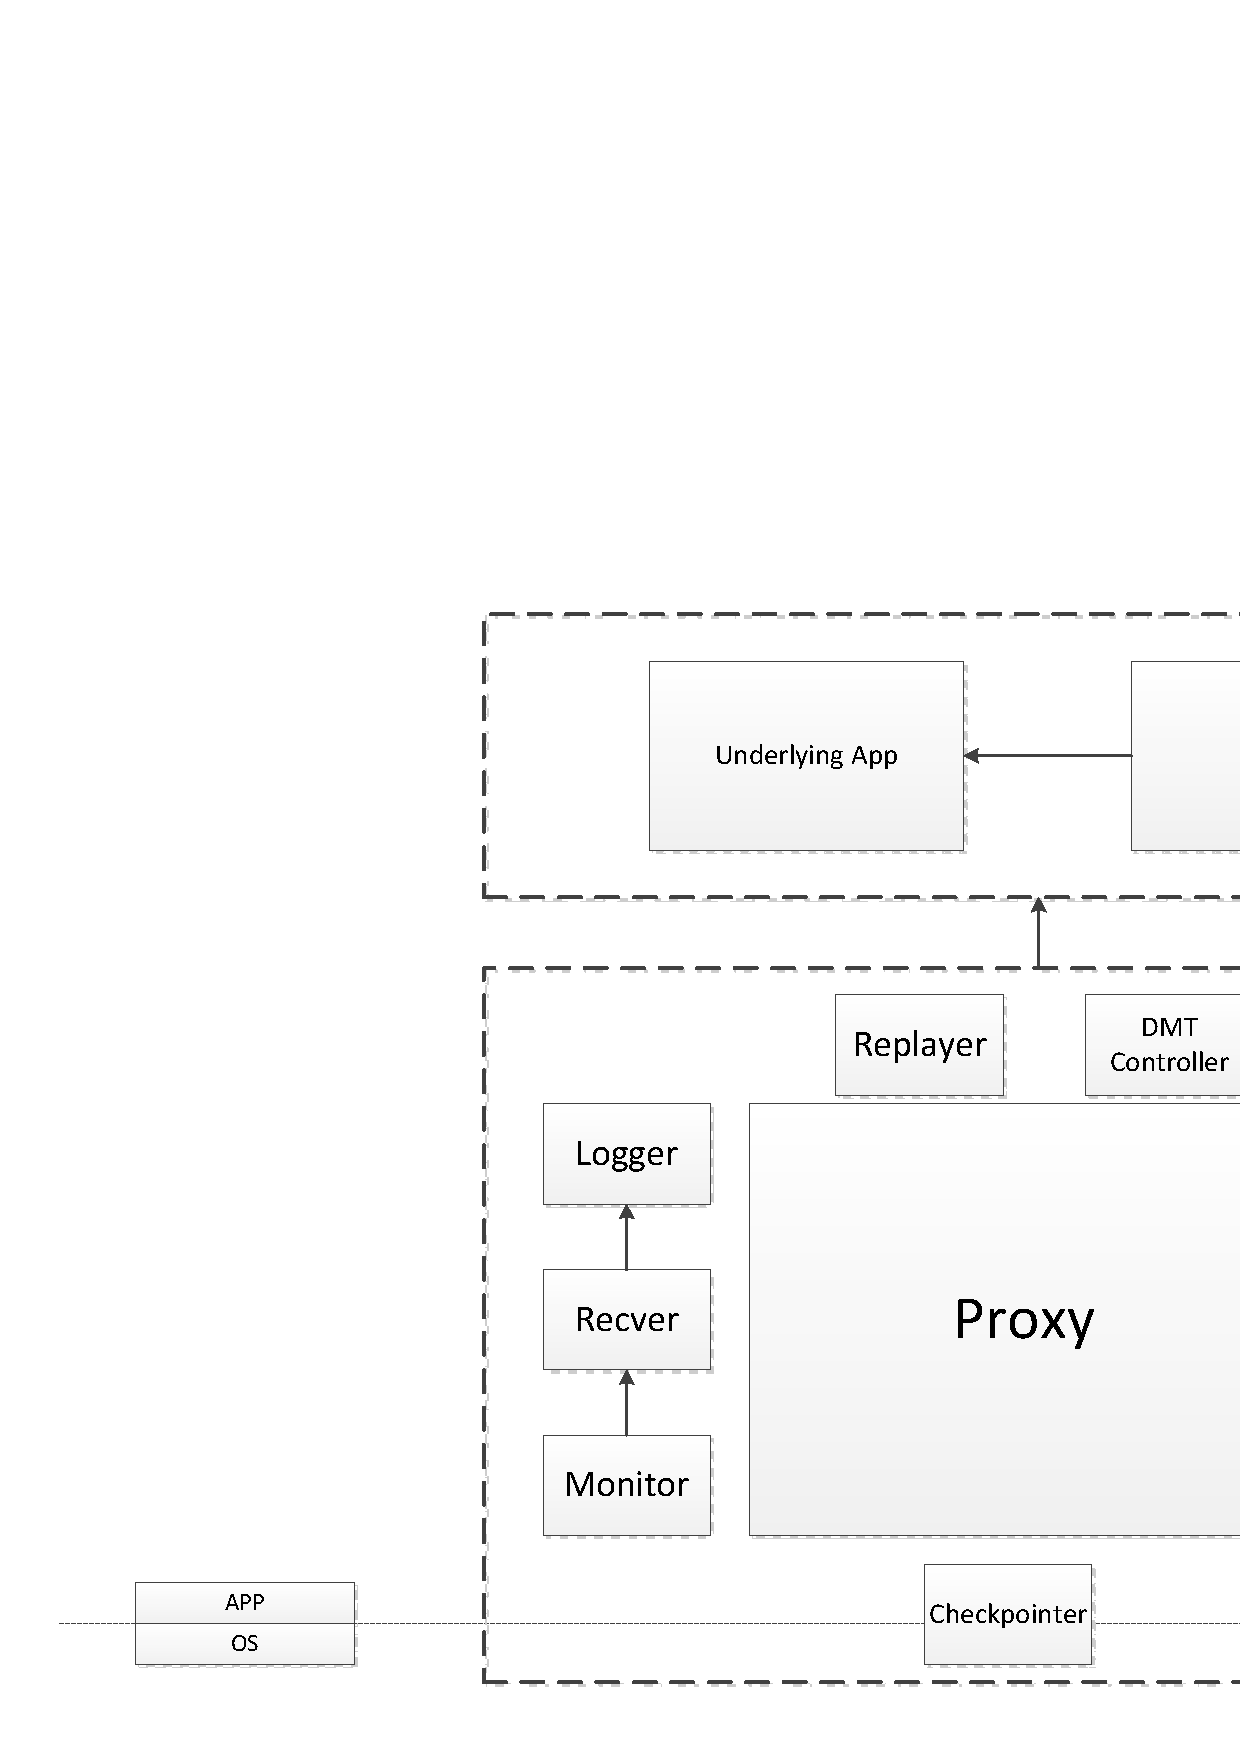
\includegraphics[width=0.4\textwidth]{figures/architecture}
\vspace{-.05in}
\caption{{\em \msmr architecture.}} \label{fig:arch}
\vspace{-.05in}
\end{figure}


\subsubsection{Systems configuration} \label{sec:rep-config}

Two key things: nodes, and the pattern of servrers. We support two modes, 
point-to-point (or P2P) mode (pairwised send() and recv()) and group mode (a number of send() 
and one select()).

\subsubsection{Reaching consensus on socket APIs} \label{sec:rep-consensus}
The key goal of our consensus module is: ensure all replicas execute the same 
sequence of socket operations in the same total order, and each operation must 
be executed (or returned) at the same logical time. To achieve this goal, we 
leverage \paxos to performance the consensus on socket operations, and 
logical clocks are carried as value of each consensus instance. Therefore, our 
consensus module is transparent to \paxos logic and enjoy the same fault tolerance 
benefits as \paxos.

Because we focus on replicating application states on the server side, not the 
whole client-server system, we only need to support blocking socket operations at server side
that depend on external network inputs. Here are a rich set of popular 
blocking socket operations we support: recv()/read(), accept(), select(), poll(), and 
epoll().

One challenge for reaching consensus for blocking socket operations is: neither the proxy nor 
the \smt module can know what operations a server is going to execute (we can 
not passively block all blocking operations on the server side and then ask for 
consensus, because this may be too slow; we want to perform consensus upfront 
and concurrently). Fortunately, each of these blocking operations must 
correspond to an event at the ``client" side (in \msmr, the proxy is the client 
that sends requests to the server). At the proxy side, there are only three 
operations interacting with the servers: send(), connect(), and close(). 
Depending on the pattern in the configuration file (\S\ref{sec:rep-config}), we 
handle the blocking operations in server side with these two patterns:

(1) P2P mode. When the proxy sees a connect() operation from the client, it invokes a 
consensus instance with accept(). When the proxy sees a send() operation from the client, it 
invokes a consensus instance with recv(). The logical clock in these consensus 
are just value and won't affect \paxos logic. We will discuss how to calculate 
the logical clock in (\S\ref{sec:rep-interface}).

(2) Group mode. This mode involves select() and a set of send()/connect() 
operations. Let's take select() as example, and handling poll() and epoll() are 
similar. Handling this mode is challenging, because we we need to make sure 
all replicas execute the same sequence (including timing) of 
select() operations with mixed use of recv() and accetp(), with each call 
the same set of send()/connect() operations. And we need to handle select() 
timeouts. In order to address this challenge, we come up with a really simple 
and clean design: in this mode, we actually only need to handle select(), 
because in this mode both recv() and accetp() become non-blocking (so they do 
not need any consensus and do not consume any logical clocks). In the 
proxy of the primay, we batch the send()/connect() operations with a fixed 
number N (usually this is the number of CPU cores) or an adaptable timeout (a 
configurable value, and we currently make it an order of magnitude smaller than the 
average response time of the server), and for each batch of these operations, 
we invoke a \paxos instance with select(). And for these batch of requests, we 
also invoke them on other replicas (as \paxos value). Timeout of select() is 
not a problem, because our \smt wrappers change the timeout to be forever.

Todo: data format of our operations. Operation ID, arguments, logical clocks, 
etc. This is not critical because all these are just \paxos consensus value.

\subsubsection{Interaction of Consensus and \smt} \label{sec:rep-interface}

The key of making sure all replicas execute blocking socket operations at the 
same timing is ensuring the same logical clocks for each of these operations. 
One key challenge is how to ensure a predicted logical clock is 
feasible (\ie after a predicted logical clock has reach consensus, it must be 
still feasible in the primary as well as the replicas). For example, we must 
consider at least these scenario: a network thread that executes 
accept()/recv() may have Pthreads synchronization between two recv() operations.
And each of the \paxos operations must leave enough logical clock gaps for 
worker threads to make progress. Also, the logical clock gap bewteen two \paxos 
operations have performance impact: if the gap is too small, the could be lots 
requests got received but few are served; if the gap is too big, there may be 
more requests served but few are received.

We introduce our runtime algorithm that address this challenge. The key idea is 
combining both our \smt run queue/wait queue and the \paxos operation queue to 
ensure each \paxos operation is scheduled at the same logical timing at each 
replica. Specifically, we need to maintain %% introduce two hints: task\_start(), tast\_end() the number of idle worker thread (or n\_idle) and
the number of socket connections (or n\_conn). Below is the 
algorithm rules:

(1) Core rule: all recv() or select() operations are treated as blocking calls and the 
threads calling these functions will wait for a global \smt turn, and be put into wait 
queue. When there is a matcing \paxos operation at the head of the \paxos 
queue, this thread will be put back from the wait queue to the run queue.

\begin{figure}[t]
\centering
\begin{minipage}{.5\textwidth}
\lgrindfile{code/msmr-wait-rule.cpp.lineno}
\end{minipage}
\vspace{-.1in}
\caption{{\em The synchronization rule algorithm.}} \label{fig:msmr-wait-rule}
\vspace{-.05in}
\end{figure}

(2) Synchronization rule (Figure~\ref{fig:msmr-wait-rule}): this rule synchronizes the \paxos queue with the 
\smt run queue and wait queue. When ever an operation is scheduled (and executed) at the \smt run queue 
head, if the wait que has threads waiting for \paxos operations, current thread does busy wait until
this condition is true: the \paxos queue is not empty, 
or the number of connection from client to proxy is 0; and then, if the \paxos 
queue is not empty, if it finds a 
corresponding server thread in the wait queue, it dequeues the head \paxos operation, 
and put this thread into the head of the run 
queue, and then let the thread execute the \paxos operation. 

Analysis on the wait rule: First, checking the \paxos queue is not 
empty is critical, because sometimes some operatios arrive at some replicas 
faster than that at some other replicas, but whenever the \paxos queue is not 
empty, the \smt runtime ``observes" a deterministic \paxos queue, and
we can safely ensure the same order for these \paxos operations.
Note that if the wait queue has no threads waiting for \paxos operation, the 
run queue head does not need to wait for the \paxos queue to be non empty at 
all, which could reducd performance impact of the ``waiting for \paxos queue to be not empty".
Second, the ``corresponding" above is easy to maintain because we see the socket pair mapping from 
both proxy and server side, and this mapping is initially established by seeing 
a connect() operation from a thread in the proxy side and find a server thread blocking at accept() 
operation in the wait queue, and then increment n\_conn by 1. Also, waiting for the 
condition guarantee to move forward because we have the termination rule below.

(3) Connection termination rule: if current \paxos operation is close(), then 
we decrement n\_conn by 1. Also, if 
the proxy can not ping to the client within a timeout limit, the proxy also 
marks the client as dead and sends a close() to the server.

%% This is an optimization (not for correctness), because waiting for the 
%% \paxos queue to be not empty can still slow down the whole system if there is 
%% only one thread listening on new connections but all incoming requests are from 
%% existing connections. In this scenario, each lock/unlock while serving 
%% requests must wait for the \paxos queue to be not empty, which may be very slot.
%% This performance problem can be mitigated by: if currently no all worker 
%% threads are serving requests (n\_idle is 0), even if \paxos queue is not empty, 
%% we still do not serve this \paxos operation (and this is still a feasible 
%% execution because the server can ``pretend" that the requests do not come).

%% (4) Hint rule: task\_start() and tast\_end() are treated as normal non-blocking and 
%% totally ordered \smt operations, and we decrease and increase n\_idle when 
%% these functions are called respectively. These two hints are easy to add to 
%% mark the working region of worker threads, and they are very critical to 
%% performance: for each operation at the run queue head, if n\_idle is greater 
%% than 0, and the \paxos queue is not empty, then just dequeues the \paxos 
%% operation from \paxos queue head, and then picks the corresponding server thread 
%% to the run queue head. This is an optimization: otherwise (\ie, we serve recv() 
%% and sync operations in a RR fashion), if serving a request 
%% requres lots of sync operations within each worker thread, we may have many 
%% more accumulated received requests before the worker threads can finish serving one batch 
%% of requests.

%% Actually, for a sequence of operations that requre \paxos, we only need to make 
%% sure the (n+1)th event has a logical clock larger than the nth event by 2. 
%% Larger is sufficient because event current server is serving requests, as long 
%% as we reach a consensus for the (n+1)th operation, the \smt runtime will just 
%% simply schedule this operation by blocking the threads serving requests (or 
%% worker threads), which 
%% does not affect runtime correctness (despite some perfomrance impact). It has 
%% to be larger than 2, because larger than 1 will prevent the worker threads from 
%% making any progress if there are an infinite number of network inputs.

%% As a demonstration of the above point, let's consider this extreme case: there are an
%% infinite number of network inputs, and each worker thread serving exiting 
%% request must do a very large number of requests (let's say one billion locks, 
%% but it must be finite). As long as each of the \paxos operations has a logical 
%% clock gap (\ie, larger than 2), then as the input sequence comes, the worker 
%% thread should have enough chance to finish (although it may be very slot), 
%% guaranteeing forward progress.

\subsection{Read-only optimization} \label{sec:rep-readonly}
For speed, modern SMR systems introduce read-only optimization: for many applications such as web servers and key-value stores,
 most of read operations do not modify applcation states, and SMR systems process them rapidly in 
local replicas without reaching consensus for these operations. Todo: needs a 
carefuly definition of read-only requests, because we only have schedule hash 
and we can not monitor shared memory variables.

Unfortunately, in the multithreading settings, some read-only requests such as http GET requests may
modify the application's internal cache, potentially causing divergence of both application states and 
schedules on processing these requests.

In order to support read-only optimizations in \msmr, we leverage the performance critical 
section (a.k.a pcs) in \parrot~cite{parrot:sosp13}, so that we could process 
these read-only operations rapidly without needing consensus. Todo: also 
mention the client side design for identifying read-only requests.

In order to address the above challenge that read-only reqeusts may modify internal 
application cache and causing schedule divergence, we leverage a key 
insight: although the first few of them may modify application's internal states, this 
sequence tend to make the application finally converge to a stable state. Based 
on this insight, we could design an approach to soundly detect the application 
state changes by checking the schedule hash serving current request, and 
safely roll back to a 'soft' checkpoint if we detect state changes and 
deliver these first few read requests to the primary. Our approach can soundly 
detect application state changes (including even application internal cache 
expiration) that may affect schedules. And this approach enables our system 
to be very fast: run even faster than the single node un-replicated 
application.

Although this read-only optimization approach is simple and sound, it has to 
address a few challenges. First, although the internal cache modified by read-only 
requests may affect the schedules of read or write requests. Second, the 
soundness of this approach should not be weakened by corner case events in the 
distributed systems.

In order to address the first challenge (\ie, read-only requests may affect 
other read or write requests), our key approach is: maintain schedule hash for write 
requests. We consider all these four cases:

(1) The same (input) read requests affecting themselves. This is avoided by 
having the schedule hash for read-only requests, as mentioned above.

(2) Read requests affecting write requests. For each ``accept" message of a 
write request sent by the \paxos primary node, we attach the schedule hash (for 
the first operation, it is empty, and this has no conflict) of 
the last executed operation in the this ``accept" message with the ``committed" 
view stamp, so that all the replicas can compare this schedule hash with its 
own ones after executing each request. This carefuly design does not require 
the primary to execute the current request first, get the schedule hash, and 
then start consenses, because we attach the previous schedule hash. Once a 
replica executes a write request, and founds that the current schedule hash is 
different from the ones sent from the primary, current replica just rolls back 
to a soft checkpoint and then replays only requests that require consenses (the 
replica can safely ignore read-only requests). We expect this roll back is 
rare, because the application internal cache tends to be a per-input property 
and should rarely affect other inputs.

(3) Read requests affecting other read requests. This can also be detected by 
the schedule hash for each read request, because schedule hash is the unique ``stable" 
signature of each read request, and once some read requests are affected by 
other read requests, their schedule hash becomes different.

(4) Write affect read. For this case, we may need more than two read-only 
operations to be involved in consensus, but this is fine, as read-only requests 
are majority of requests and they tend to push the system to converge to a 
stable state.

One may ask, can we just simply maintain schedule hash for write requests and 
simply roll back when we see a divergence of schedule hash for each write 
request? This naive approach could work, if and only if our marking of read 
only requests are completely precise (\ie, it would never mark write request as 
read-only requests). Unfortunately, this case could not be completely avoided 
because human may make mistakes, and the self comparisons of read-only requests 
are the key to detect whether they are actually read-only requests (\eg, some 
requests marked as read-only may actually modify systems states everytime and 
their schedule hash may never converge).

To address the second challenges, we discuss our approach on three (Todo: more?) popular 
corner cases:

(1) Packet loss causing schedule hash to get lost. This won't occur, because 
for each node in \msmr, the consensus proxy and the application shares the same 
physical machine, and the schedule hash executed by the application is recorded 
persistently by us.

(2) Node crash. For this case, in the restart phase, we simply erase all 
schedule hash, because current in memory application state does not match the 
application memmory states implied in schedule hash any more. Note that 
schedule hash is just our hints, and it can be safely erased in any case 
without affecting soundness or correctness of our system.

(3) Network partition or \paxos message lost. In this case, we can do nothing 
special (but we can still serve requests, \eg, read-only requests), because 
later if the network gets back, our above schedule hash can detect all types of 
read/write conflicts and roll back; if the network never gets back, this node 
can not reach any consensus with other nodes and then won't execute any write 
requests.

%% One may ask, can we just maintain the schedule hash for the write requests 
%% only, and then just simply roll back when we see a divergence of the schedule 
%% hash? Yes, this is a correct design, but it may trigger lots of roll backs, 
%% because the first few read only requests may cause the logical clock  ??? Not 
%% really.


\subsection{Implementation} \label{sec:rep-impl}
TBD.

\subsubsection{Checkpointing and failure recovery} \label{sec:rep-checkpoint}
In order to recover a replica from failure or application conflicts caused by 
read only requests, we need to have a systematic checkpoint mechanisms for the applications.

In order to ensure both robustness against failures and speed over conflicts, 
\msmr designs two kinds of checkpoints: to handle node failures, a hard checkpoint saves current application 
state permanently to 
disk; to handle conflicts, a soft checkpoint saves current application state by 
simply forking a process (issue: can this fork clone all child threads?), and 
rolling back to a soft checkpoint just simply changes the forked process as 
current working process.

A hard checkpoint is expensive because of disk IO. In order to minimize its 
impact, we have a replica (instead of a primary that needs to serve requests 
and get back to client as soon as possible) to do a periodical (minutes or hours) checkpiont. This 
hard checkpoint operation is first handled as a \paxos consensus operation (the 
ID of this checkpoint is the last executed \paxos operation in current 
replica, and the location of the checkpoint is the replica's ID), and then performs a hard checkpoint.
Once any node in the distributed 
system is restarted, it simply checks the last checkpoint in the \paxos 
operation log and asks for a network transformation of the checkpoint, and 
then replays the following operations. Since node failures are rare, we expect 
this mechanism won't affect performance much. In the implementation level, We can have a dedicated
client in the system to periodical asks for hard checkpoints.

A soft checkpoint is invoked more frequently (\eg, in seconds) than a hard 
checkpoint, and it is just a local property for resolving conflicts (\ie, it will never 
be transmitted across nodes).

Todo: for short checkpoints, how can we implement a fork with child threads?

Currently our checkpoint for application involves four things: file systems, memory state,
network sockets, and CPU registers. For file systems, we use Dockers.
For memory state, we use virtual machine or hardware virtualization 
techniques. Network sockets can also easily checkpointed because the network 
sockets between the applications (\eg, servers) and our proxy are controled by 
us internally. CPU registers can also be saved.

\subsubsection{Handling nondeterministic operations} \label{sec:rep-nondet}
In reality, applications may call nondetermnistic operations, including 
``rand()" and ``gettimeofday()", and the return value of these functions may 
affect control flow and schedules of applications (\eg, the \apache uses 
``gettimeofday()" to check cache expiration). We use the same approach as that 
in PMP (todo: add citation) to address this problem: for each request, a \msmr roxy executes
this function multiple times (long enough) in advance and send the result list to all the replicas,
replicas just take the result from the list to serve the request from the 
application. For ``rand()", we acutally execute the ``srand()" and enforce the 
same seeds on all replicas.

\subsubsection{Maintaining systems resources} \label{sec:re-resource}
Systems resources such as file descriptors may need to be maintained by 
\msmr and we maintain their own mappings and return a consistent value to the 
return value of IO functions.

\subsubsection{Maintaining systems resources} \label{sec:rep-race}
We have a dedicated client to invoke a race detector on a replica node within our system, 
and we don't forward read-only requests for this replica. This detector is to 
practically remind develpers to fix and diagnose races.

\subsection{Evaluation plan} \label{sec:rep-eval}
Performance overhead with the single node multithreaded version.

Performance breakdown (analysis) of the consensus component and the read-only optimization component.

Race detection results.

Recovery scenarios and performance results.

Systems parameter sensitivity evaluation, including the periods of hard and soft checkpoints, etc.


\subsection{\msmr has broad applications} \label{sec:rep-apps}

This section describes several potential applications of \msmr.

\subsubsection{Fast and effective concurrency error detection} \label{sec:rep-races} 
TBD.

\subsubsection{Fast information flow tracking} \label{sec:rep-ift}
TBD.

\subsubsection{TBD} \label{sec:rep-apps-tbd}
TBD.

